\documentclass[conference]{IEEEtran}
\usepackage{booktabs} 
\IEEEoverridecommandlockouts
\usepackage{cite}
\usepackage{amsmath,amssymb,amsfonts}
\usepackage[T1]{fontenc}
\usepackage{newtxtext}
\usepackage{graphicx}
 
\usepackage{placeins}
\usepackage{textcomp}
\usepackage{xcolor}
\usepackage{subcaption} 
\usepackage{romannum}
\usepackage{array}
\usepackage{url}
\usepackage{float}
\def\BibTeX{{\rm B\kern-.05em{\sc i\kern-.025em b}\kern-.08em
    T\kern-.1667em\lower.7ex\hbox{E}\kern-.125emX}}

% Auto-generated by teramove_eval/make_assets.py -- do not edit.
\newcommand{\CommEmptyCov}{93.3}
\newcommand{\ConvGFinal}{1.360}
\newcommand{\ConvHFinal}{1.405}
\newcommand{\ConvPFinal}{1.429}
\newcommand{\ConvSeeds}{30}
\newcommand{\DenBeforeA}{79.9}
\newcommand{\DenBeforeB}{82.1}
\newcommand{\DenBeforeC}{77.1}
\newcommand{\DenBeforeD}{75.0}
\newcommand{\DenCovDiffG}{-0.9}
\newcommand{\DenCovDiffP}{-3.3}
\newcommand{\DenCovGapG}{0.9}
\newcommand{\DenCovGapP}{3.3}
\newcommand{\DenDispRedG}{84.9}
\newcommand{\DenDispRedP}{79.0}
\newcommand{\DenGCovA}{99.0}
\newcommand{\DenGCovAll}{95.5}
\newcommand{\DenGCovB}{96.9}
\newcommand{\DenGCovC}{95.6}
\newcommand{\DenGCovD}{93.2}
\newcommand{\DenGCovPval}{=0.13}
\newcommand{\DenGDispA}{75.1}
\newcommand{\DenGDispAll}{45.7}
\newcommand{\DenGDispB}{47.2}
\newcommand{\DenGDispC}{41.4}
\newcommand{\DenGDispD}{37.3}
\newcommand{\DenGDispPval}{<0.001}
\newcommand{\DenHCovA}{97.2}
\newcommand{\DenHCovAll}{94.6}
\newcommand{\DenHCovB}{96.6}
\newcommand{\DenHCovC}{93.9}
\newcommand{\DenHCovD}{92.9}
\newcommand{\DenHDispA}{4.3}
\newcommand{\DenHDispAll}{6.9}
\newcommand{\DenHDispB}{8.3}
\newcommand{\DenHDispC}{6.3}
\newcommand{\DenHDispD}{7.2}
\newcommand{\DenPCovA}{99.7}
\newcommand{\DenPCovAll}{97.9}
\newcommand{\DenPCovB}{98.5}
\newcommand{\DenPCovC}{97.8}
\newcommand{\DenPCovD}{96.8}
\newcommand{\DenPCovPval}{<0.001}
\newcommand{\DenPDispA}{64.4}
\newcommand{\DenPDispAll}{32.9}
\newcommand{\DenPDispB}{31.2}
\newcommand{\DenPDispC}{27.5}
\newcommand{\DenPDispD}{26.4}
\newcommand{\DenPDispPval}{<0.001}
\newcommand{\DenTrigA}{10}
\newcommand{\DenTrigAll}{75}
\newcommand{\DenTrigB}{18}
\newcommand{\DenTrigC}{19}
\newcommand{\DenTrigD}{28}
\newcommand{\FigFourAfter}{91.3}
\newcommand{\FigFourBefore}{84.3}
\newcommand{\FigFourDisp}{1.2}
\newcommand{\FigFourTier}{3}
\newcommand{\HungHu}{7.9}
\newcommand{\HungNN}{8.4}
\newcommand{\HungP}{=0.18}
\newcommand{\HungSaving}{0.5}
\newcommand{\HungSavingPct}{6.0}
\newcommand{\MilpEmptyCov}{61.9}
\newcommand{\SensACov}{94.0}
\newcommand{\SensADisp}{19.3}
\newcommand{\SensBCov}{94.6}
\newcommand{\SensBDisp}{12.1}
\newcommand{\SensCCov}{93.9}
\newcommand{\SensCDisp}{17.0}
\newcommand{\SensCovMax}{94.6}
\newcommand{\SensCovMin}{93.9}
\newcommand{\SensDCov}{94.2}
\newcommand{\SensDDisp}{16.0}
\newcommand{\SensDispMax}{19.3}
\newcommand{\SensDispMin}{12.1}
\newcommand{\SensMinP}{0.16}
\newcommand{\SeqBeforeA}{62.8}
\newcommand{\SeqBeforeB}{90.6}
\newcommand{\SeqBeforeC}{79.6}
\newcommand{\SeqCovGapMax}{1.1}
\newcommand{\SeqDispRedG}{91.2}
\newcommand{\SeqDispRedP}{81.6}
\newcommand{\SeqGCovA}{96.3}
\newcommand{\SeqGCovAvg}{94.4}
\newcommand{\SeqGCovB}{95.5}
\newcommand{\SeqGCovC}{91.3}
\newcommand{\SeqGCovPval}{=0.72}
\newcommand{\SeqGDispA}{63.9}
\newcommand{\SeqGDispB}{63.4}
\newcommand{\SeqGDispC}{54.9}
\newcommand{\SeqGDispPval}{<0.001}
\newcommand{\SeqGDispTot}{182.3}
\newcommand{\SeqGReach}{88.9}
\newcommand{\SeqGReachA}{100.0}
\newcommand{\SeqGReachB}{93.3}
\newcommand{\SeqGReachC}{73.3}
\newcommand{\SeqHCovA}{94.8}
\newcommand{\SeqHCovAvg}{94.2}
\newcommand{\SeqHCovB}{95.6}
\newcommand{\SeqHCovC}{92.1}
\newcommand{\SeqHDispA}{9.5}
\newcommand{\SeqHDispB}{1.8}
\newcommand{\SeqHDispC}{4.7}
\newcommand{\SeqHDispTot}{16.0}
\newcommand{\SeqHReach}{97.8}
\newcommand{\SeqHReachA}{100.0}
\newcommand{\SeqHReachB}{100.0}
\newcommand{\SeqHReachC}{93.3}
\newcommand{\SeqPCovA}{98.4}
\newcommand{\SeqPCovAvg}{95.3}
\newcommand{\SeqPCovB}{94.8}
\newcommand{\SeqPCovC}{92.6}
\newcommand{\SeqPCovPval}{=0.03}
\newcommand{\SeqPDispA}{40.0}
\newcommand{\SeqPDispB}{25.7}
\newcommand{\SeqPDispC}{21.2}
\newcommand{\SeqPDispPval}{<0.001}
\newcommand{\SeqPDispTot}{86.9}
\newcommand{\SeqPReach}{90.0}
\newcommand{\SeqPReachA}{100.0}
\newcommand{\SeqPReachB}{86.7}
\newcommand{\SeqPReachC}{83.3}
\newcommand{\SeqTierFourA}{43}
\newcommand{\SeqTierFourB}{3}
\newcommand{\SeqTierFourC}{30}
\newcommand{\SeqTierLowA}{0}
\newcommand{\SeqTierLowB}{97}
\newcommand{\SeqTierLowC}{37}
\newcommand{\TierBase}{82.9}
\newcommand{\TierDispFour}{7.9}
\newcommand{\TierDispThree}{1.6}
\newcommand{\TierDispTwo}{0.0}
\newcommand{\TierFour}{96.9}
\newcommand{\TierFourReach}{96.7}
\newcommand{\TierGainFour}{4.0}
\newcommand{\TierGainThree}{5.6}
\newcommand{\TierGainTwo}{4.4}
\newcommand{\TierSeeds}{30}
\newcommand{\TierThree}{92.9}
\newcommand{\TierTwo}{87.3}
\newcommand{\TierTwoShare}{31.4}


\begin{document}

\title{TeraMove: Context-Aware Reconfiguration of THz Access Points for Resilient Pervasive Connectivity}

\author{\IEEEauthorblockN{Author 1, Author 2, Author 3}
\IEEEauthorblockA{Department of Computer Science and Engineering, Indian Institute of Technology Bhilai, India}}

\maketitle


\begin{abstract}
The Terahertz (THz) band promises high-speed indoor
connectivity for 6G, but its dependence on line-of-sight
makes it highly vulnerable to dynamic blockages. Traditional indoor deployments rely on static Access Points (APs) and cannot adapt when physical obstructions arise
or crowd patterns shift, leading to low coverage. In this
paper, we present TeraMove, a blockage-aware framework that
uses spatial human-density context to detect THz link degradation
from dynamic blockages and adapt the AP configuration to restore
pervasive connectivity. We describe how this context can be obtained from 3D LiDAR depth sensing; our evaluation uses a synthetic clustered crowd-density model.
TeraMove first establishes an optimal baseline layout for AP placement using a Mixed Integer Linear Programming (MILP) model over 3D
coordinates and beam orientations, then employs a four-tier optimization that escalates from electronic beam steering to full 3D
node repositioning, performing physical movement only when lighter
adaptations prove insufficient to provide threshold coverage.
Evaluations in a realistic indoor environment, averaged over 30 runs, show that crowd-induced
blockages reduce density-weighted coverage to \SeqBeforeA\%; TeraMove restores it to \SeqHCovA\%. Over three successive crowd configurations, TeraMove meets the 90\% coverage target in \SeqHReach\% of the adaptation steps, against \SeqPReach\% for a standard particle swarm optimizer and \SeqGReach\% for a genetic algorithm. It also moves APs \SeqDispRedP\% and \SeqDispRedG\% less than these two baselines.
\end{abstract}

\begin{IEEEkeywords}
THz Communication, Context-Aware Adaptation, Pervasive Connectivity, Spatio-Temporal Blockage Modeling, Adaptive Infrastructure, HPSO, Dynamic Repositioning
\end{IEEEkeywords}

\section{Introduction}

The emergence of 6G networks is driven by a new class of applications, holographic communication, immersive extended reality, and digital twins, that demand sustained multi-Terabit-per-second data rates with ultra-low latency, far exceeding what current 5G infrastructure can deliver. The Terahertz (THz) band (0.1--10~THz), with orders of magnitude more available spectrum than sub-6~GHz or millimeter-wave (mmWave) bands, is widely regarded as the enabling physical layer for this next generational leap. However, THz signals suffer extreme path loss and molecular absorption, forcing transmitters to use narrow, highly directional beams that require an unobstructed Line-of-Sight (LoS) to every user. In populated indoor spaces, this LoS dependence is inherently fragile: a single human body crossing the beam can cause attenuation exceeding 20~dB, enough to collapse the link entirely.

The straightforward solution is static placement optimization, fixing transmitting nodes at predetermined positions to maximize coverage of the people in the building. Existing methods typically treat this as a 2D problem at a uniform ceiling height. While adequate for an empty floor plan, such deployments assume the propagation environment never changes. However, dynamic blockages caused by human mobility continuously reshape the interference landscape, and a layout providing near-perfect user coverage at one moment can suffer severe degradation when a crowd clusters unexpectedly. 
Depth sensing offers a highly reliable means to obtain such changing environmental context. Recent advancements in solid-state 3D LiDAR have shown that accurate human tracking and counting in indoor environments \cite{b27,b29}. Such sensing can provide the spatial human-density context needed to reason about changing blockage conditions. Static over-provisioning cannot anticipate every future crowd pattern and can lead to very high costs.

We present \textit{TeraMove}, a context-aware framework that treats transmitting node deployment as a continuous adaptation problem rather than a one-time placement. TeraMove uses a spatial human-density representation to characterize dynamic blockage and first applies a Mixed-Integer Linear Programming (MILP) formulation to minimize the number of deployed transmitting nodes while satisfying coverage and SINR constraints. When crowd shifts degrade user coverage below a threshold, it triggers an Hierarchical Particle Swarm Optimization (HPSO) engine with a 4-tier cascading architecture: Tier~1 checks whether action is needed; Tier~2 electronically adjusts beam azimuth and beamwidth at zero physical cost; Tier~3 permits minor height changes; Tier~4, as a last resort, enables full 3D repositioning. In our evaluation, Tier~2 alone provides \TierTwoShare\% of the coverage gain of the full cascade, at zero physical cost. A Hungarian algorithm-based assignment further minimizes aggregate physical displacement when movement is unavoidable.

Although focused on THz, the framework is transmitter-agnostic and applies equally to mmWave small cells, Wi-Fi access points, or 5G base stations, anywhere LoS-dependent links face dynamic blockages. We use the term ``Access Points'' (APs) throughout, noting the methodology extends naturally across deployment paradigms.

The main \textbf{contributions} of this paper are:
\begin{itemize}
    \item A MILP formulation that jointly optimizes 3D AP coordinates and azimuth orientations under a complete THz channel model, minimizing the number of nodes needed to guarantee user-level SINR coverage.

    \item An HPSO algorithm for real-time dynamic repositioning, with a composite fitness function that prioritizes human-density-weighted coverage while penalizing unnecessary physical displacement.

    \item A 4-tier cascading architecture that escalates from electronic beam steering to full spatial repositioning only when needed, significantly recovering user coverage while minimizing total physical node displacement compared to alternative approaches.
\end{itemize}











\section{Related Work}

The THz band (0.1--10~THz) offers very large bandwidth for 6G, but
suffers from high path loss, molecular absorption, and severe
line-of-sight (LoS) blockage~\cite{b5,b1,b2}. Human bodies can cause
more than 20~dB attenuation~\cite{b6}, while pedestrian density and
mobility strongly affect THz outage and SINR~\cite{b3,b14}. These
characteristics make static deployments vulnerable to
spatiotemporally varying human blockage.

Existing AP placement methods primarily optimize the network before
deployment. Baswade~\textit{et al.}~\cite{b4} formulated base-station
placement using mixed-integer optimization, while LoS-coverage maximization with multiple mmWave APs was studied by Liu~\textit{et
al.}~\cite{b7}. Such approaches provide effective initial layouts but do
not adapt the deployment after propagation conditions change. PSO and
its variants have also been applied to wireless optimization,
including 3D UAV-BS placement~\cite{b15} and mmWave massive-MIMO
beamforming~\cite{b16}.However, these approaches mainly focus on optimizing placement or communication parameters, rather than combining electronic adaptation with physical AP reconfiguration when human blockage changes.
Physical mobility offers another means of adapting wireless coverage as user locations vary. Wireless platforms based on UAV can adjust their position in three dimensions to improve coverage and optimize their trajectories~\cite{b15,b20}. Similarly, movable APs have been studied for indoor WLANs, where the AP locations are changed according to user distribution~\cite{b21}. Movable antennas further exploit spatial channel variations by dynamically changing antenna positions
~\cite{b22}. Nevertheless, these approaches do not jointly consider
indoor THz beam adaptation, vertical AP adjustment, and progressive
full-3D repositioning based on human blockage.

Dynamic adaptation also requires information about human
movement. Vision-based learning has been used to predict impending
mmWave/THz blockages~\cite{b25}.
Specifically, 3D LiDAR point clouds have been extensively explored for high-resolution indoor crowd counting and geometry tracking~\cite{b27,b29}. These sensing approaches can provide the spatial
human-density information required for blockage-aware adaptation,
but existing work does not directly couple such contextual
information with hierarchical AP reconfiguration that escalates from
electronic beam adaptation to physical 3D repositioning.














\section{System Model and Problem Formulation}

Designing indoor Terahertz (THz) networks requires strategic placement of APs to ensure reliable coverage. The positioning must account for the building's permanent structural layout as well as the random movement of people within it. The key notations used throughout this paper are given in Table~\ref{tab:notations}.


\renewcommand{\arraystretch}{1.3}

\setlength{\tabcolsep}{3pt} 

\begin{table}[htbp]
  \centering
  \caption{Glossary of Proposed Model}
  \label{tab:notations}

  \begin{tabular}{@{} l >{\raggedright\arraybackslash}p{0.72\linewidth} @{}}
    \toprule
    \textbf{Notation} & \textbf{Definition} \\
    \midrule
    $\mathcal{U}, \mathcal{A}$ & Set of target user locations and candidate AP locations \\
    $d_{u,a}$ & 3D Euclidean distance between $u$ and $a$ (meters) \\
    $d_{u,a}^{2D}, d_{u,c}^{2D}$ & 2D projected distances on the horizontal plane (meters) \\
    $\phi_a$ & Azimuth pointing direction (orientation) of AP $a$ \\
    $\Delta\phi$ & Angular deviation between user location and AP orientation \\
    $\theta_{\text{HPBW}}$ & Half-Power Beamwidth of the directional THz antenna \\
    $h_{\text{human}}$ & Average physical height of a human blocker  \\
    $z(c)$ & Interpolated elevation of the signal beam at grid cell $c$ \\
    $W_a \in \{0,1\}$ & 1 if an AP is deployed at location $a$, 0 otherwise \\
    $Y_{u,a} \in \{0,1\}$ & 1 if user $u$ is associated with AP $a$, 0 otherwise \\
    $\eta$ & Target coverage threshold parameter (ratio, e.g., 0.90) \\
    $f$ & Operating frequency (Hz) \\
    $c$ & Speed of light (m/s) \\
    $k(f)$ & Molecular absorption coefficient at frequency $f$ \\
    $D_h(c)$ & Normalized human density score at grid cell $c$ \\
    $P_{\text{tx}}, P_{\text{rx}}$ & Transmit and received signal power (dBm) \\
    $G_{\text{tx}}, G_{\text{rx}}$ & Transmit and receive antenna gains (dBi) \\
    $G_{\text{max}}, G_{\text{min}}$ & Main-lobe peak gain and side-lobe leakage floor (dBi) \\
    $\text{SINR}_{\text{th}}$ & Minimum required SINR in each target sub-region \\
    $N_0$ & System noise floor (linear scale) \\
    $L_{w}$ & Penetration penalty for static walls (dB) \\
    $L_{h}$ & Penetration penalty for human blockages (dB) \\
    Inf & An arbitrarily large positive constant \\
    \midrule
    $v_i^{(t)}, x_i^{(t)}$ & Velocity and position of HPSO particle $i$ at iteration $t$ \\
    $w$ & Inertia weight (linearly decreasing from $0.9$ to $0.4$) \\
    $c_1, c_2$ & Cognitive and social learning factors \\
    $p_i^{\text{best}}$ & Personal best position of particle $i$ \\
    $g^{\text{best}}$ & Global best position discovered by the swarm \\
    $F$ & Composite fitness score of a candidate AP configuration \\
    $R_{\text{cell}}$ & Ratio of grid cells meeting the SINR threshold \\
    $R_{\text{density}}$ & Ratio of covered human density to total density \\
    $B$ & Bonus awarded when target coverage is achieved \\
    $M$ & Normalized movement penalty for physical displacement \\
    $C_p$ & Anti-clustering penalty for AP spatial diversity \\
    $w_c, w_d$ & Coverage and density weights in fitness function \\
    $\beta, \gamma$ & Displacement and clustering penalty coefficients \\
    $\mathcal{R}_{\text{prev}}, \mathcal{R}_{\text{new}}$ & Sets of current and optimized AP positions \\
    $C_{ij}$ & Displacement cost to move AP $r_i$ to new position $r'_j$ \\
    $\sigma^*$ & Optimal AP-to-position assignment (Hungarian) \\
    \bottomrule
  \end{tabular}
\end{table}

\renewcommand{\arraystretch}{1.0}
\setlength{\tabcolsep}{6pt}

The indoor environment is discretized into a 3D volumetric grid. Let $\mathcal{U}$ denote the set of target user equipment locations requiring coverage, and let $\mathcal{A}$ denote the set of candidate AP locations. Unlike traditional 2D placement models, we explicitly optimize over the vertical Z-axis to accurately model signal propagation. Let the 3D coordinates of the user device $u$ be $(x_u, y_u, z_u)$ and the candidate AP $a$ be $(x_a, y_a, z_a)$. The volumetric Euclidean distance $d_{u,a}$ is calculated as:
\begin{equation}
    d_{u,a} = \sqrt{(x_u - x_a)^2 + (y_u - y_a)^2 + (z_u - z_a)^2}
    \label{eq:3d_distance}
\end{equation}
where the user height $z_u$ is fixed to a standard level, and the optimization algorithm selects an optimal AP mounting elevation $z_a$ from a discrete set of candidate heights. 

This 3D distance $d_{u,a}$ denotes the fundamental free-space propagation. The base Free Space Loss (FSL) for a signal operating at frequency $f$ over distance $d_{u,a}$ is derived from the Friis transmission equation:
\begin{equation}
    PL_{\text{FSL}}(d_{u,a}) = 20\log_{10}\left(\frac{4\pi f d_{u,a}}{c}\right)
\end{equation}
where $c$ is the speed of light in a vacuum. The total deterministic (line-of-sight) path loss $PL_{\text{LoS}}(u,a)$ for a THz link further incorporates molecular absorption loss and static attenuation \cite{b1}:
\begin{equation}
    PL_{\text{LoS}}(u,a) = PL_{\text{FSL}}(d_{u,a}) + PL_{\text{ABS}}(d_{u,a}) + L_{\text{static}}
    \label{eq:total_pl}
\end{equation}
where $PL_{\text{FSL}}(d_{u,a})$ represents the free-space path loss, $L_{\text{static}}$ denotes the attenuation penalty from static infrastructure, and $PL_{\text{ABS}}(d_{u,a})$ accounts for atmospheric molecular absorption at high frequencies \cite{b2}, calculated in dB as:
\begin{equation}
    PL_{\text{ABS}}(d_{u,a}) = 4.343 \cdot k(f) \cdot d_{u,a}
\end{equation}
with $k(f)$ representing the frequency-dependent molecular absorption coefficient.

Due to the highly directional nature of THz signals, line-of-sight (LoS) obstructions severely degrade link quality. We model two distinct types of blockages: static infrastructure and dynamic human mobility. For static obstacles, let $\mathcal{W}$ denote the set of walls within the environment. If the 3D line segment connecting $u$ and $a$ intersects a wall $w \in \mathcal{W}$, a material-specific penetration penalty $L_{w}$ (e.g., concrete, wood, glass) is accumulated:
\begin{equation}
    L_{\text{static}} = \sum_{w \in \mathcal{W}_{\text{intersect}}} L_{w}
\end{equation}

Furthermore, THz signals suffer severe attenuation when occluded by human bodies \cite{b3}. We define an expected dynamic loss based on the normalized human density score $D_h(c) \in [0,1]$ for each grid cell (computed in Section~IV-A) over the set of grid cells $\mathcal{C}_{u,a}$ intersected by the 2D projection of the link.  A human only obstructs the signal if the elevation of the beam $z(c)$ as it passes through cell $c$ drops below 
the standard human height $h_{\text{human}}$.  
This geometrical threshold is equivalent to the critical blockage distance limits derived from similar triangles in prior work on THz blockages for humans. Using linear interpolation based on 2D traversed distance $d_{u,c}^{2D}$ and total 2D distance $d_{u,a}^{2D}$, the beam elevation at cell $c$ is given as:
\begin{equation}
    z(c) = z_u + \frac{d_{u,c}^{2D}}{d_{u,a}^{2D}} (z_a - z_u)
\end{equation}
The expected dynamic blockage loss is then defined using an indicator function $\mathbb{I}(\cdot)$, which equals 1 if the beam strikes the human body and 0 otherwise:
\begin{equation}
    L_{\text{dynamic}} = \sum_{c \in \mathcal{C}_{u,a}} D_h(c) \cdot L_{h} \cdot \mathbb{I}\Big(z(c) \le h_{\text{human}}\Big)
    \label{eq:dynamic_loss}
\end{equation}
where $L_{h}$ is the empirical penalty caused by human blockage.

To overcome extreme path loss, THz networks use highly directional antennas rather than omnidirectional antennas. We adopt a flat-top sector antenna model parameterized by the half-power beamwidth (HPBW), $\theta_{\text{HPBW}}$, and the AP's mounting azimuth orientation $\phi_a$. Although our model specifically analyzes the horizontal beamwidth, we assume that APs above the users ($z_a > z_u$) are optimally angled downward. This downward tilt ensures the main signal beam reaches the users directly. As a result, we can simplify our analysis by calculating the signal gain only in the horizontal~plane. 

Let $\phi_{u,a}$ denote the azimuth of user $u$ as seen from AP $a$. Both $\phi_{u,a}$ and the AP orientation $\phi_a$ are compass bearings, measured clockwise from North ($+y$), which is the convention of the MILP layout. The shortest angular deviation $\Delta\phi$ between the user's location and the AP's orientation, is calculated as:
\begin{equation}
    \Delta\phi = \big|(\phi_{u,a} - \phi_a + 180^{\circ}) \bmod 360^{\circ} - 180^{\circ}\big|
    \label{eq:ang_dev}
\end{equation}
This angular deviation ($\Delta\phi$) determines the transmit gain $G_{\text{tx}}(\Delta\phi)$ applied to the link:
\begin{equation}
    G_{\text{tx}}(\Delta\phi) = 
    \begin{cases} 
      G_{\text{max}}, & \text{if } \Delta\phi \le \frac{\theta_{\text{HPBW}}}{2} \\
      G_{\text{min}}, & \text{otherwise}
    \end{cases}
    \label{eq:beamwidth}
\end{equation}
where $G_{\text{max}}$ is the gain in the main signal direction, and $G_{\text{min}}$ represents the small amount of signal leakage in other directions. In our evaluation, $G_{\text{max}}$ is held fixed at 30~dBi across all evaluated beamwidths (Table~\ref{tab:sim_params}); incorporating the physical gain--beamwidth trade-off is left to future work. $G_{\text{min}}$ is modeled as practically negligible, meaning the signal drops significantly outside the HPBW. The total path loss $PL(u,a)$ experienced by a link combines the deterministic LoS component with the expected dynamic human blockage:
\begin{equation}
    PL(u,a) = PL_{\text{LoS}}(u,a) + L_{\text{dynamic}}(u,a)
    \label{eq:total_pl_combined}
\end{equation}
Finally, the received power $P_{\text{rx}}^{(u,a)}$ (in linear scale) is obtained from the total path loss and the antenna gain as:
\begin{equation}
    P_{\text{rx}}^{(u,a)} = 10^{\frac{P_{\text{tx}} + G_{\text{tx}}(\Delta\phi) + G_{\text{rx}} - PL(u,a) - 30}{10}}
\end{equation}

\section{Proposed Work}

Our objective is to ensure that every user within the indoor environment receives a minimum required SINR ($\text{SINR}_{\text{th}}$) using the fewest THz APs possible, even as human crowds dynamically reshape the blockage landscape. We address this in two stages: first, we formulate the static baseline placement as a MILP to compute an optimal initial deployment over a discretized candidate set; second, we introduce an HPSO-based dynamic repositioning framework with a 4-tier cascading architecture to adapt the deployment in real time when crowd shifts degrade user coverage.

\subsection{Context Acquisition from Human-Density Sensing}

	TeraMove uses spatial human-density information to capture changes in the blockage environment. In practice, this contextual data is obtained using 3D LiDAR sensors, which generate real-time topographical point clouds of the room. The raw 3D point cloud is divided into the exact volumetric grid cells ($c$) used by our formulation. By subtracting the static background, we isolate dynamic points corresponding to humans or moving furniture. The human density score $D_h(c) \in [0,1]$ for a specific vertical column is calculated as:
	\begin{equation}
		D_h(c) = \min \left(1, \frac{N_{\text{dyn}}(c)}{N_{\text{max}}} \right)
	\end{equation}
	where $N_{\text{dyn}}(c)$ is the number of dynamic LiDAR points detected in the vertical column at cell $c$, and $N_{\text{max}}$ is the expected maximum number of points for a single human body. In our evaluation, we generate the equivalent human-density map synthetically (Section~\ref{sec:setup}) to evaluate coverage and trigger AP adaptation when needed.



\subsection{Static Baseline Placement via MILP}

We formulate the baseline optimization problem as a Mixed-Integer Linear Programming (MILP) model. The primary objective is to minimize the total number of APs deployed, expressed by Eq. \eqref{eq:objective}:
\begin{equation}
    \min \sum_{a \in \mathcal{A}} W_a
    \label{eq:objective}
\end{equation}

Eq. \eqref{eq:assoc1} ensures that each target sub-region is associated with exactly one deployed AP. Eq. \eqref{eq:assoc2} mandates that a user $u$ can only logically associate with a candidate location $a$ if an AP is physically deployed there ($W_a = 1$).
\begin{equation}
    \sum_{a \in \mathcal{A}} Y_{u,a} = 1, \quad \forall u \in \mathcal{U}
    \label{eq:assoc1}
\end{equation}
\begin{equation}
    Y_{u,a} \le W_a, \quad \forall u \in \mathcal{U}, \forall a \in \mathcal{A}
    \label{eq:assoc2}
\end{equation}

In practical deployment scenarios where satisfying 100\% coverage is physically or economically infeasible, Eq. \eqref{eq:assoc1} is relaxed to an inequality ($\sum_{a \in \mathcal{A}} Y_{u,a} \le 1$), and a global coverage constraint is introduced. Let $\eta \in (0,1]$ denote the required proportion of the total environment that must be served. To strictly enforce this spatial coverage ratio, the total number of successfully associated sub-regions must satisfy the following constraint:
\begin{equation}
    \sum_{u \in \mathcal{U}} \sum_{a \in \mathcal{A}} Y_{u,a} \ge \eta |\mathcal{U}|
    \label{eq:coverage_constraint}
\end{equation}
where $|\mathcal{U}|$ represents the total number of target user sub-regions in the partitioned grid.

The next constraint is to maintain the minimum SINR \textit{i.e.}, threshold in each sub-region considering multi AP interference. Eq. \eqref{eq:sinr} ensures that the minimum SINR is maintained in each sub-region:
\begin{equation}
    \frac{P_{\text{rx}}^{(u,a)} + \text{Inf} \cdot (1 - Y_{u,a})}{N_0 + \sum_{\substack{b \in \mathcal{A} \\ b \ne a}} P_{\text{rx}}^{(u,b)} W_b} \ge \text{SINR}_{\text{th}}, \quad \forall u \in \mathcal{U}, a \in \mathcal{A}
    \label{eq:sinr}
\end{equation}

The Left Hand Side (LHS) of Eq. \eqref{eq:sinr} is the ratio of received signal power from the AP to which the user is associated, to the sum of system noise $N_0$ and interference from other deployed APs. When the $u^{\text{th}}$ user is associated with an AP located at $a$, $Y_{u,a} = 1$. So, the term $\textit{Inf} \cdot (1 - Y_{u,a})$ goes to zero, and the LHS of Eq. \eqref{eq:sinr} has to satisfy the constraint. Otherwise, if $Y_{u,a} = 0$, the term $\textit{Inf} \cdot (1 - Y_{u,a})$ takes on an arbitrarily large value. Because of this term, the numerator becomes extremely large and inherently satisfies the inequality, effectively ignoring the constraint for unassociated links \cite{b4}. The term $\textit{Inf} \cdot (1 - Y_{u,a})$ is needed because a single AP might not provide the minimum SINR to all sub-regions in the building simultaneously; this formulation ensures the overall feasibility of the MILP equations. 

The above constraint can be linearized by cross-multiplying the denominator to the right-hand side. Because the candidate set $\mathcal{A}$ enumerates discrete (position, height, azimuth) tuples, $P_{\text{rx}}^{(u,b)}$ is a precomputed constant for each $(u,b)$ pair and $W_b$ is a binary decision variable; their product $P_{\text{rx}}^{(u,b)} W_b$ is therefore inherently linear. The linearized form of Eq.~\eqref{eq:sinr} is
\begin{equation}
\begin{split}
    P_{\text{rx}}^{(u,a)} + \text{Inf} \cdot (1 - Y_{u,a}) &\ge \text{SINR}_{\text{th}} \cdot \Big( N_0 + \sum_{\substack{b \in \mathcal{A} \\ b \ne a}} P_{\text{rx}}^{(u,b)} W_b \Big), \\
    &\quad \forall u \in \mathcal{U}, a \in \mathcal{A}
\end{split}
\label{eq:sinr_linear}
\end{equation}
This equivalent formulation ensures that the entire optimization problem remains within the MILP framework, enabling standard solvers to compute optimal AP deployments over the discretized candidate set.


\subsection{Dynamic AP Repositioning via HPSO}

The MILP formulation produces an optimal AP layout for the discretized candidate set in a given static environment. However, indoor human crowds are inherently dynamic, and a deployment optimized for one crowd configuration may become suboptimal minutes later. Rather than deploying additional APs for every possible crowd pattern, we propose dynamically repositioning the existing APs to track the evolving human density landscape.

To accomplish this, we employ a Hierarchical Particle Swarm Optimization (HPSO) algorithm built on the standard velocity-update formulation of \cite{b11,b13}, with the hierarchy realized through the tiered activation of search dimensions described below rather than through evolutionary-state-based parameter adaptation. HPSO is a population-based metaheuristic where a swarm of candidate solutions (particles) explores the search space cooperatively. Each particle maintains a position vector $x_i$ encoding the AP configuration parameters and a velocity vector $v_i$ governing its exploration trajectory. The swarm evolves over $T$ iterations according to the velocity update rule:
\begin{equation}
    v_i^{(t+1)} = w \cdot v_i^{(t)} + c_1 r_1 (p_i^{\text{best}} - x_i^{(t)}) + c_2 r_2 (g^{\text{best}} - x_i^{(t)})
    \label{eq:pso_velocity}
\end{equation}
where $w$ is the inertia weight that linearly decreases from $0.9$ to $0.4$ over the course of optimization to transition from exploration to exploitation, $c_1$ and $c_2$ are cognitive and social learning factors (both set to $1.5$), $r_1, r_2 \sim U(0,1)$ are random coefficients, $p_i^{\text{best}}$ is the personal best position of particle $i$, and $g^{\text{best}}$ is the global best position discovered by the entire swarm. The position is subsequently updated as $x_i^{(t+1)} = x_i^{(t)} + v_i^{(t+1)}$, with per-dimension velocity clamping to prevent divergence.

The fitness function that guides the swarm combines multiple objectives into a single composite score:
\begin{equation}
    F = w_c \cdot R_{\text{cell}} + w_d \cdot R_{\text{density}} + B - \beta \cdot M - \gamma \cdot C_p
    \label{eq:fitness}
\end{equation}
where $R_{\text{cell}}$ is the ratio of grid cells meeting the SINR threshold, $R_{\text{density}}$ is the ratio of covered human density to total density, $B$ is a bonus awarded when target coverage is achieved, and $M$ is a normalized movement penalty encouraging minimal physical displacement. $C_p$ is an anti-clustering penalty that discourages APs from congregating too closely, formalized as:
\begin{equation}
    C_p = \frac{1}{n(n-1)} \sum_{i=1}^{n}\sum_{\substack{j=1 \\ j \ne i}}^{n} \max\left(0,\ 1 - \frac{\|r_i - r_j\|}{d_{\min}}\right)
    \label{eq:clustering_penalty}
\end{equation}
where $n$ is the number of deployed APs, $r_i, r_j$ are their 3D positions, and $d_{\min}$ is a minimum desired inter-AP spacing (Table~\ref{tab:sim_params}). Unless stated otherwise we use configuration~D of Table~\ref{tab:sensitivity}: the weights $w_c = 0.4$ and $w_d = 0.6$ prioritize human-centric coverage, while $\beta = 0.25$ and $\gamma = 0.3$ govern the displacement and clustering penalties, respectively. The bonus is $B=0.5$ when the density-weighted coverage reaches $\eta$, and $M$ is the total displacement divided by $n$ times the building diagonal.

\subsubsection{4-Tier Cascading Optimization Architecture}

A key design principle of our dynamic framework is the minimization of physical AP displacement. Moving APs incurs practical costs: service interruption during relocation, mechanical wear, and potential re-calibration requirements. To address this, we introduce a 4-tier cascading optimization architecture that progressively unlocks more degrees of freedom only when simpler adjustments prove insufficient.

\begin{itemize}
    \item \textbf{Tier 1 -- Baseline Evaluation:} The system evaluates the current AP configuration against the updated human density map. If the density-weighted coverage already meets the target threshold ($\ge 90\%$), no optimization is triggered. This avoids unnecessary computation and physical displacement.

    \item \textbf{Tier 2 -- Beam Parameter Optimization:} If coverage is insufficient, the HPSO optimizes only the azimuth orientation ($\phi_a$) and beamwidth ($\alpha$) of each AP. Since these are electronic adjustments requiring no physical movement, Tier~2 achieves coverage improvements at zero displacement cost.

      \item \textbf{Tier 3 -- Height Adjustment:} If Tier~2 fails to restore adequate coverage, the optimizer additionally adjusts the vertical mounting elevation ($z_a$) of each AP from the set of candidate heights. This involves minor physical adjustment along the Z-axis only.

    \item \textbf{Tier 4 -- Full Spatial Repositioning:} As a last resort, the HPSO unlocks the horizontal coordinates ($x_a, y_a$), enabling complete 3D relocation of APs. To prevent excessive displacement, one-third of the particle swarm is seeded near the current AP positions, allowing the optimizer to preferentially discover nearby solutions.
\end{itemize}

At each tier, the HPSO locks the velocity components of the dimensions not yet activated (e.g., in Tier~2, the $x$, $y$, and $z$ velocity components are clamped to zero). One particle is initialized at the current configuration, so a tier never returns a configuration with lower fitness than its input. AP positions are kept inside the building, 0.25\,m from the outer walls. This cascading structure ensures that the system always attempts the least disruptive adjustment first before escalating.

\subsubsection{Displacement Minimization via Hungarian Algorithm}

When the HPSO produces an optimized set of AP positions, a critical assignment problem arises: which \textit{existing} AP should move to which \textit{new} position? A naive assignment may result in unnecessarily large total displacement. To minimize the aggregate physical relocation distance, we formulate this as a classical assignment problem and solve it using the Hungarian algorithm \cite{b12}.

Let $\mathcal{R}_{\text{prev}} = \{r_1, \ldots, r_n\}$ denote the $n$ current AP positions and $\mathcal{R}_{\text{new}} = \{r'_1, \ldots, r'_n\}$ denote the $n$ optimized positions. We construct a cost matrix $C \in \mathbb{R}^{n \times n}$ where each entry $C_{ij}$ represents the 3D Euclidean displacement required to move existing AP $r_i$ to new position $r'_j$:
\begin{equation}
    C_{ij} = \sqrt{(x_i - x'_j)^2 + (y_i - y'_j)^2 + (z_i - z'_j)^2}
    \label{eq:cost_matrix}
\end{equation}

The Hungarian algorithm finds the optimal one-to-one assignment $\sigma^*: \{1, \ldots, n\} \to \{1, \ldots, n\}$ that minimizes the total displacement:
\begin{equation}
    \sigma^* = \arg\min_{\sigma} \sum_{i=1}^{n} C_{i, \sigma(i)}
    \label{eq:hungarian}
\end{equation}
This assignment is computed in $O(n^3)$ time, which is negligible for the typical number of indoor APs ($n \le 30$).
\section{Experimental Setup and Simulation Results}\label{sec:setup}
We consider an academic environment based on a representative university department floor ($32\,\text{m}\times20\,\text{m}\times3\,\text{m}$, 1\,m grid).
Human-density maps are generated synthetically.
$N_c$ circular crowd clusters of radius 2\,m (default $N_c=9$) are placed with uniformly random centres, and $D_h(c)$ decays linearly from 1 at a cluster centre to 0 at its rim (the maximum is taken where clusters overlap).
The three time steps $t_0$, $t_1$ and $t_2$ use three independent draws of this model.
The simulation parameters are summarized in Table~\ref{tab:sim_params}.

We use $\text{SINR}_{\text{th}}=5$\,dB because it is the minimum signal quality for reliable THz link establishment with low-order modulation (e.g., QPSK)~\cite{b5}.
The primary metric is the density-weighted coverage $R_{\text{density}}$: the share of human density located in grid cells with SINR at or above the threshold.
Every statistic is the mean over 30 independent runs, reported with a 95\% Student-$t$ confidence interval.
Paired differences between methods are tested with the Wilcoxon signed-rank test.
The swarm has $S=50$ particles and runs $T=20$ iterations per tier.

\begin{table}[t]
\centering
\caption{Simulation Parameters}\label{tab:sim_params}
\footnotesize
\begin{tabular}{@{}lp{0.5\columnwidth}@{}}
\toprule
Parameter & Value\\
\midrule
Environment & $32\times20\times3$\,m, 1\,m grid\\
Operating frequency $f$ & 300\,GHz\\
Transmit power $P_{\text{tx}}$ & 20\,dBm\\
Main-lobe gain $G_{\text{max}}$ & 30\,dBi (all beamwidths)\\
Side-lobe leakage $G_{\text{min}}$ & $-100$\,dBi (negligible)\\
Receive gain $G_{\text{rx}}$ & 0\,dBi\\
Beamwidths $\theta_{\text{HPBW}}$ & $30^\circ, 45^\circ, 60^\circ, 75^\circ, 90^\circ, 120^\circ$\\
AP heights $z_a$ & 2.0--3.0\,m, 0.2\,m steps\\
Azimuths $\phi_a$ & $45^\circ$ steps, compass bearing\\
User height $z_u$ & 1.0\,m\\
Noise floor $N_0$ & $-64$\,dBm (10\,GHz, NF 10\,dB)\\
Absorption $k(f)$ & $1.54\times10^{-3}$\,m$^{-1}$ (6.68\,dB/km~\cite{itur676,iturpy})\\
Wall penalties $L_w$ & concrete 30, wood 20, glass 15\,dB\\
Cubicles & 1.0\,m high, 20\,dB\\
Human blocker $L_h$ & 20\,dB, height 1.6\,m\\
Coverage target $\eta$ & 0.90\\
$\text{SINR}_{\text{th}}$ & 5\,dB\\
Swarm & $S=50$, $T=20$ per tier, $w$: $0.9\to0.4$\\
Runs & 30 independent seeds\\
\bottomrule
\end{tabular}
\end{table}

\subsection{Static Baseline Deployment}
In the MILP study~\cite{milp}, the solver needs 14 APs to reach 100\% coverage at $\text{SINR}_{\text{th}}=5$\,dB under its channel model ($P_{\text{tx}}=10$\,dBm, $G_{\text{max}}=24$\,dBi, $G_{\text{min}}=-5$\,dBi).
Candidate elevations from 2.0 to 3.0\,m in 0.2\,m steps let the APs transmit above the 1.0\,m cubicles.
The MILP study also reports the following:
\begin{itemize}
\item Raising $\text{SINR}_{\text{th}}$ from 1 to 5\,dB increases the AP count from 9 to 10 for 90\% coverage.
\item Wide beams ($90^\circ$--$120^\circ$) need only 10 APs for 90\% coverage, whereas narrow beams ($60^\circ$--$75^\circ$) need 15.
\end{itemize}

The simulator used in this paper has the parameters of Table~\ref{tab:sim_params}, which differ from the MILP's channel model.
Under these parameters, the MILP layout with $60^\circ$ beams covers \MilpEmptyCov\% of the empty floor.
We therefore commission the layout once for the empty floor.
The AP positions stay unchanged, and the heights, azimuths and beamwidths are tuned by exhaustive per-AP coordinate descent.
This raises empty-floor coverage to \CommEmptyCov\% (Fig.~\ref{fig:static}), and the commissioned layout is the starting configuration of every experiment.

\begin{figure}[t]
\centering
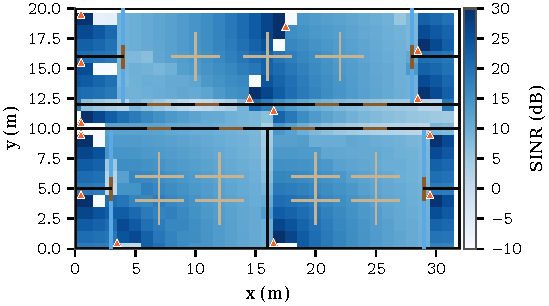
\includegraphics[width=\columnwidth]{figures/static_sinr.pdf}
\caption{SINR of the commissioned 14-AP layout on the empty floor (triangles: APs); \CommEmptyCov\% of the grid cells reach 5\,dB.}
\label{fig:static}
\end{figure}

\subsection{Tier-wise Coverage and Displacement Analysis}
To measure what each tier contributes, we force all tiers to run on 30 crowd maps ($N_c=9$) starting from the commissioned layout (Table~\ref{tab:tiers}, Fig.~\ref{fig:tiers}).
Crowds reduce the density-weighted coverage to \TierBase\% on average.
Tier~2 raises it by \TierGainTwo{} percentage points (pp) to \TierTwo\% with no movement.
Tier~3 adds \TierGainThree\,pp for \TierDispThree\,m of vertical movement.
Tier~4 adds a final \TierGainFour\,pp, at \TierDispFour\,m of cumulative displacement, and ends at \TierFour\%.
Tier~2 thus provides \TierTwoShare\% of the total gain at zero physical cost.
In operation, the cascade stops at the first tier that reaches $\eta$ (Section~\ref{sec:temporal}), so Tiers~3 and~4 run only when needed.

When movement is required, the Hungarian assignment yields \HungHu\,m of total displacement after Tier~4, against \HungNN\,m for a nearest-neighbour assignment.
That is \HungSavingPct\% less, but the difference is not statistically significant in our setting ($p\HungP$).

\begin{table}[t]
\centering
\caption{Tier-wise Coverage and Displacement (mean over 30 crowds; 95\% CI on coverage)}\label{tab:tiers}
\footnotesize
\setlength{\tabcolsep}{3pt}
\begin{tabular}{@{}lrrr@{}}
\toprule
Tier & Coverage (\%) & Gain (pp) & Cum.\ displ.\ (m)\\
\midrule
Baseline (Tier 1) & 82.9$\pm$3.8 & -- & 0.0 \\
Tier 2 (beams) & 87.3$\pm$3.4 & 4.4 & 0.0 \\
Tier 3 (+ height) & 92.9$\pm$2.7 & 5.6 & 1.6 \\
Tier 4 (+ position) & 96.9$\pm$1.2 & 4.0 & 7.9 \\
\bottomrule
\end{tabular}

\end{table}

\begin{figure}[t]
\centering
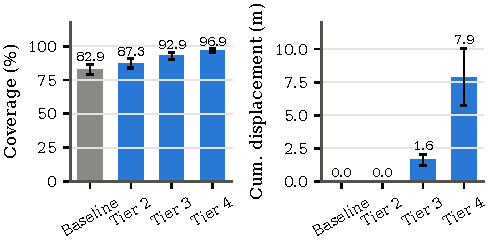
\includegraphics[width=\columnwidth]{figures/tiers.pdf}
\caption{Coverage (left) and cumulative displacement (right) after each tier (mean, 95\% CI over 30 crowds).}
\label{fig:tiers}
\end{figure}

\subsection{Temporal Crowd Adaptation}\label{sec:temporal}
We apply the cascade to three successive crowd configurations $t_0$, $t_1$ and $t_2$.
Each step starts from the configuration left by the previous step, and the sequence is repeated with 30 optimizer seeds.
\begin{itemize}
\item \textbf{$t_0$:} the crowd lowers coverage from the commissioned layout to \SeqBeforeA\%.
TeraMove restores it to \SeqHCovA\% with \SeqHDispA\,m of movement on average; \SeqTierFourA\% of the runs escalate to Tier~4.
\item \textbf{$t_1$:} coverage before adaptation is \SeqBeforeB\%, and \SeqTierLowB\% of the runs need at most beam steering.
Coverage after adaptation is \SeqHCovB\%, with \SeqHDispB\,m of movement.
\item \textbf{$t_2$:} coverage drops to \SeqBeforeC\% and is restored to \SeqHCovC\% with \SeqHDispC\,m of movement.
\end{itemize}
The 90\% target is met in \SeqHReachA, \SeqHReachB{} and \SeqHReachC\% of the runs at $t_0$, $t_1$ and $t_2$ (Fig.~\ref{fig:temporal}).

Fig.~\ref{fig:sequence} shows one run at $t_2$:
\begin{itemize}
\item[(a)] the configuration left by $t_1$, shown on the empty floor;
\item[(b)] its SINR under the $t_1$ crowd;
\item[(c)] the new crowd map;
\item[(d)] the degraded SINR, at \FigFourBefore\% coverage;
\item[(e)] the adapted configuration;
\item[(f)] the restored SINR, at \FigFourAfter\% coverage.
\end{itemize}
The cascade stopped at Tier~\FigFourTier{} after \FigFourDisp\,m of movement.

\begin{figure}[t]
\centering
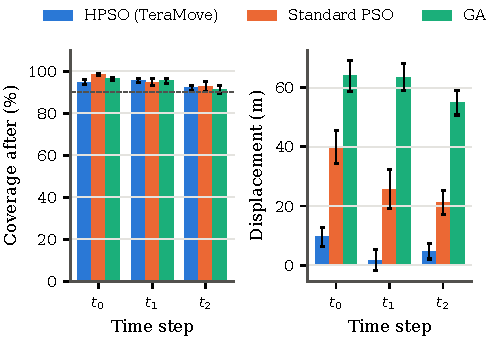
\includegraphics[width=\columnwidth]{figures/temporal.pdf}
\caption{Coverage after adaptation (left) and displacement (right) per time step (mean, 95\% CI over 30 runs); dashed line: 90\% target.}
\label{fig:temporal}
\end{figure}

\begin{figure*}[t]
\centering
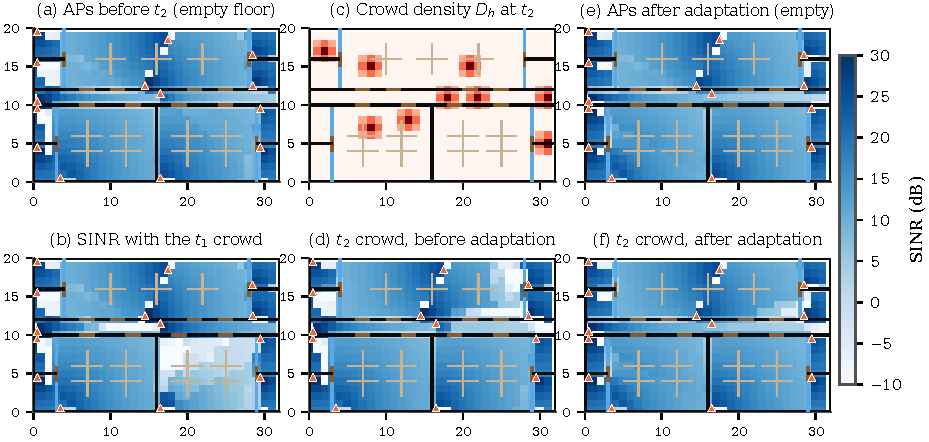
\includegraphics[width=\textwidth]{figures/sequence_t2.pdf}
\caption{Adaptation at $t_2$ (one run). (a) Configuration after $t_1$; (b) its SINR under the $t_1$ crowd; (c) $t_2$ crowd density; (d) SINR before adaptation; (e) adapted configuration; (f) SINR after adaptation. Triangles mark APs.}
\label{fig:sequence}
\end{figure*}

\subsection{Comparison with Alternative Approaches}
We compare the HPSO against a standard PSO and a genetic algorithm (GA).
We exclude combinatorial approaches such as greedy set cover: they discard the AP state reached at the previous step and treat each time step as a new problem, so they do not preserve the movement continuity that physical APs require.
\begin{itemize}
\item \textbf{Standard PSO} optimizes the same composite fitness (Eq.~\eqref{eq:fitness}, including the displacement penalty $\beta M$) without the tier hierarchy.
All coordinates and beam parameters are free from the first iteration, and the swarm is initialized uniformly.
\item \textbf{GA} is real-coded, with binary tournaments, BLX-0.5 crossover~\cite{blx} with probability 0.9, Gaussian mutation and elitism.
It checks that the improvements are not specific to PSO.
\end{itemize}
Both baselines get the cascade's worst-case budget of $3\times S\times T=3000$ evaluations.
They use the same trigger (no action if coverage is at least $\eta$), include the current configuration in their initial population, and use the Hungarian assignment.

\textbf{Temporal sequence.}
Over $t_0$--$t_2$, the HPSO moves APs \SeqHDispTot\,m in total, against \SeqPDispTot\,m for the standard PSO ($p\SeqPDispPval$) and \SeqGDispTot\,m for the GA ($p\SeqGDispPval$).
That is a reduction of \SeqDispRedP\% and \SeqDispRedG\%, respectively.
Average coverage is \SeqHCovAvg\% for the HPSO, \SeqPCovAvg\% for the standard PSO ($p\SeqPCovPval$) and \SeqGCovAvg\% for the GA ($p\SeqGCovPval$).
The standard PSO thus attains slightly higher average coverage, but it meets the 90\% target less often (\SeqPReach\% of the steps, against \SeqHReach\% for the HPSO and \SeqGReach\% for the GA).
Its shortfalls occur at $t_1$ and $t_2$ (\SeqPReachB\% and \SeqPReachC\% of the runs), after its large relocations at the previous step.

\textbf{Crowd density.}
Fig.~\ref{fig:density} varies the number of crowd clusters from 3 to 12, with 30 crowd maps per level, starting from the commissioned layout.
Only \DenTrigAll{} of the 120 maps push coverage below $\eta$ and trigger adaptation (\DenTrigA, \DenTrigB, \DenTrigC{} and \DenTrigD{} maps for 3, 6, 9 and 12 clusters).
The comparison therefore uses these events, which are identical for all methods.
On them, the HPSO reaches \DenHCovAll\% coverage.
The standard PSO reaches \DenPCovAll\%, i.e., \DenCovGapP\,pp higher ($p\DenPCovPval$), and the GA reaches \DenGCovAll\% ($p\DenGCovPval$).
To do so, the baselines move APs \DenPDispAll\,m and \DenGDispAll\,m on average, against \DenHDispAll\,m for the HPSO ($p\DenPDispPval$ and $p\DenGDispPval$).
More clusters trigger adaptation more often.
However, because the coverage metric is weighted by the density map itself, the coverage before adaptation does not fall monotonically with the number of clusters (\DenBeforeA, \DenBeforeB, \DenBeforeC{} and \DenBeforeD\%).

\textbf{Convergence.}
Fig.~\ref{fig:convergence} plots the best fitness against evaluations on the same 30 crowd maps ($N_c=9$), with all tiers forced.
The standard PSO reaches higher fitness earlier and ends at \ConvPFinal, against \ConvHFinal{} for the HPSO and \ConvGFinal{} for the GA.
The displacement penalty is normalized by $n$ times the building diagonal, so it is small compared with coverage gains, and unrestricted relocation is rewarded in fitness.
The HPSO's advantage therefore lies in how little it moves the APs, not in faster convergence.

\begin{figure*}[t]
\centering
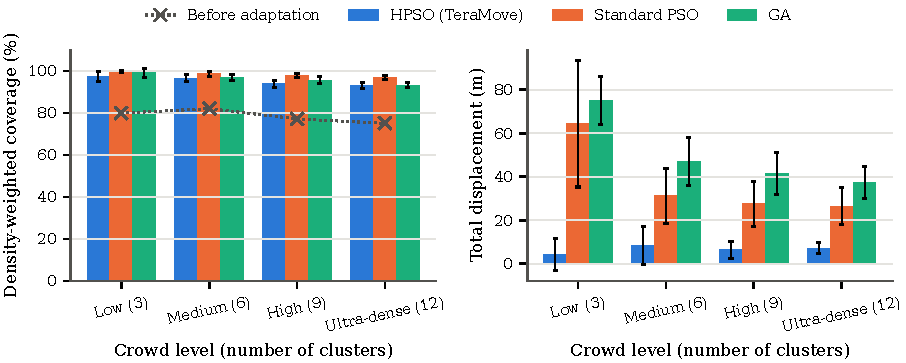
\includegraphics[width=\textwidth]{figures/density.pdf}
\caption{Coverage after adaptation (left) and total displacement (right) versus crowd level, over the events that trigger adaptation (mean, 95\% CI); crosses: coverage before adaptation.}
\label{fig:density}
\end{figure*}

\begin{figure}[t]
\centering
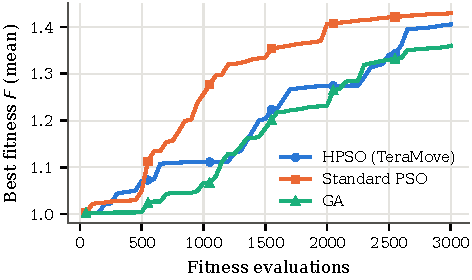
\includegraphics[width=\columnwidth]{figures/convergence.pdf}
\caption{Best fitness versus evaluations (mean over the same 30 crowd maps, budget $3\times S\times T$).}
\label{fig:convergence}
\end{figure}

\subsection{HPSO Hyperparameter Sensitivity}
Standard PSO hyperparameters (inertia weight $w$, learning factors $c_1, c_2$) follow established guidelines~\cite{b11,b13}.
To assess the domain-specific fitness weights $(w_c, w_d, \beta, \gamma)$, we run the $t_0\to t_2$ sequence with four configurations, using 30 runs each (Table~\ref{tab:sensitivity}).
All configurations reach \SensCovMin--\SensCovMax\% average coverage, and their total displacements range from \SensDispMin{} to \SensDispMax\,m.
None of the configurations A--C differs significantly from configuration D in coverage or displacement (Wilcoxon $p\ge\SensMinP$).
We therefore keep configuration D as the default: its higher movement penalty $\beta=0.25$ expresses the design preference for electronic adaptation.

\begin{table}[t]
\centering
\caption{Fitness Weight Sensitivity over $t_0\to t_2$ (mean, 95\% CI over 30 runs)}\label{tab:sensitivity}
\footnotesize
\setlength{\tabcolsep}{3pt}
\begin{tabular}{@{}lrrrrrr@{}}
\toprule
Config. & $w_c$ & $w_d$ & $\beta$ & $\gamma$ & Avg.\ cov.\ (\%) & Total disp.\ (m)\\
\midrule
A & 0.4 & 0.6 & 0.15 & 0.3 & 94.0$\pm$0.6 & 19.3$\pm$8.3 \\
B & 0.3 & 0.7 & 0.15 & 0.3 & 94.6$\pm$0.5 & 12.1$\pm$2.9 \\
C & 0.4 & 0.6 & 0.15 & 0.1 & 93.9$\pm$0.7 & 17.0$\pm$6.0 \\
D & 0.4 & 0.6 & 0.25 & 0.3 & 94.2$\pm$0.6 & 16.0$\pm$7.3 \\
\bottomrule
\end{tabular}

\end{table}

\section{Discussion}
The practical deployment of this framework can follow two operational paradigms: real-time reactive adaptation or scheduled time-based adaptation.

\textbf{Real-time adaptation.}
Here the HPSO framework runs as an active control loop integrated into the building's IoT infrastructure.
This requires real-time crowd sensing, such as camera-based tracking, Wi-Fi probe requests or infrared occupancy sensors, to keep the human-density map current.
Whenever a crowd shift drops the network below the 90\% coverage threshold, the HPSO triggers immediately.
Tier~2 corrects part of the blockage electronically, without physical motion.
The robotic mounting tracks (Tiers~3 and~4) are unlocked only when software adjustment is insufficient.

\textbf{Scheduled adaptation.}
Human mobility in large indoor environments such as universities or offices often follows predictable routines (e.g., morning arrivals, lunch hours, class changeovers).
Network operators can use historical footfall data to predict density at specific hours instead of relying on real-time tracking.
The HPSO pre-computes the configuration for each routine crowd pattern, and the APs execute the stored repositioning and beam steering at the scheduled time.

\textbf{Mechanical realization.}
Tier~3 height adjustments can use linear actuators or servo-driven vertical rail mounts attached to ceiling tracks.
Tier~4 needs ceiling-mounted robotic rail systems with bidirectional tracks, with power-over-Ethernet cable chains or retractable reels that keep power and backhaul connected during movement.
The Hungarian assignment keeps each reconfiguration cycle at the minimum total travel distance for the chosen positions, which limits mechanical wear.

\textbf{Limitations and future work.}
\begin{itemize}
\item The MILP enforces single-AP association. Multi-connectivity and re-association before physical reconfiguration would likely recover some coverage at zero mechanical cost.
\item The dynamic blockage model (Eq.~\eqref{eq:dynamic_loss}) applies an additive penalty without a saturation cap. It is a conservative bound on signal degradation, not a precise model of overlapping bodies.
\item $G_{\text{max}}$ is held at 30\,dBi for every beamwidth, so the physical gain--beamwidth trade-off is not modeled.
\item The crowd maps are synthetic, and successive time steps are independent draws rather than a mobility trace.
\item APs may move anywhere on the floor during Tier~4, so the travel paths of a real rail system are not modeled.
\item Mechanical actuation latency is not modeled, so Tiers~3 and~4 are best interpreted as scheduled rather than instantaneous adaptations.
\end{itemize}

\section{Conclusion}
This paper presented a framework for THz Access Point deployment that bridges the gap between static placement and unpredictable indoor crowds.
A 3D MILP formulation provides the baseline layout.
Because static layouts degrade when moving crowds block high-frequency signals, we introduced a human-density representation of the blockage and a 4-tier hierarchical PSO.
The HPSO escalates from zero-movement electronic beam steering to full 3D repositioning only when necessary.

In simulation, TeraMove restores density-weighted coverage from \SeqBeforeA\% to \SeqHCovA\% after a dense crowd shift.
It meets the 90\% target in \SeqHReach\% of the adaptation steps, and it moves APs \SeqDispRedP\% less than a standard PSO and \SeqDispRedG\% less than a GA, with an average coverage within \SeqCovGapMax\,pp of both.
Reliable THz networks need not rely on installing ever more APs: a fixed set of APs can be adapted to the crowds they serve, with physical movement kept to a minimum.

\begin{thebibliography}{00}
\bibitem{b1} T. S. Rappaport \textit{et al.}, ``Millimeter Wave Mobile Communications for 5G Cellular: It Will Work!,'' \textit{IEEE Access}, vol.~1, pp.~335--349, 2013.
\bibitem{b2} Y. Niu \textit{et al.}, ``A survey of millimeter wave communications (mmWave) for 5G: opportunities and challenges,'' \textit{Wireless Networks}, vol.~21, pp.~2657--2676, 2015.
\bibitem{b3} M. Gapeyenko \textit{et al.}, ``On the Temporal Effects of Mobile Blockers in Urban Millimeter-Wave Cellular Scenarios,'' \textit{IEEE Trans. Veh. Technol.}, vol.~66, no.~11, pp.~10124--10138, 2017.
\bibitem{b4} A. M. Baswade, S. Kiran M. R., B. R. Tamma, and A. Franklin, ``On Placement of LAA/LTE-U Base Stations in Heterogeneous Wireless Networks,'' in \textit{Proc. 19th Int. Conf. Distributed Computing and Networking (ICDCN)}, 2018, pp.~37:1--37:10.
\bibitem{b5} I. F. Akyildiz, J. M. Jornet, and C. Han, ``Terahertz band: Next frontier for wireless communications,'' \textit{Physical Communication}, vol.~12, pp.~16--32, 2014.
\bibitem{b6} B. A. Bilgin, H. Ramezani, and O. B. Akan, ``Human Blockage Model for Indoor Terahertz Band Communication,'' in \textit{Proc. IEEE ICC Workshops}, 2019, pp.~1--6.
\bibitem{b7} Y. Liu, Y. Jian, R. Sivakumar, and D. M. Blough, ``Maximizing Line-of-Sight Coverage for mmWave Wireless LANs With Multiple Access Points,'' \textit{IEEE/ACM Trans. Netw.}, vol.~30, no.~2, pp.~698--716, 2022.
\bibitem{b11} J. Kennedy and R. Eberhart, ``Particle swarm optimization,'' in \textit{Proc. IEEE ICNN}, 1995, vol.~4, pp.~1942--1948.
\bibitem{b12} H. W. Kuhn, ``The Hungarian method for the assignment problem,'' \textit{Naval Research Logistics Quarterly}, vol.~2, no.~1--2, pp.~83--97, 1955.
\bibitem{b13} Y. Shi and R. Eberhart, ``A modified particle swarm optimizer,'' in \textit{Proc. IEEE ICEC}, 1998, pp.~69--73.
\bibitem{b14} V. Petrov, M. Komarov, D. Moltchanov, J. M. Jornet, and Y. Koucheryavy, ``Interference and SINR in Millimeter Wave and Terahertz Communication Systems With Blocking and Directional Antennas,'' \textit{IEEE Trans. Wireless Commun.}, vol.~16, no.~3, pp.~1791--1808, 2017.
\bibitem{b15} M. Alzenad, A. El-Keyi, F. Lagum, and H. Yanikomeroglu, ``3-D Placement of an Unmanned Aerial Vehicle Base Station (UAV-BS) for Energy-Efficient Maximal Coverage,'' \textit{IEEE Wireless Commun. Lett.}, vol.~6, no.~4, pp.~434--437, 2017.
\bibitem{b16} T. A. Kareem, M. A. Hussain, and M. K. Jabbar, ``Particle Swarm Optimization Based Beamforming in Massive MIMO Systems,'' \textit{Int. J. Interact. Mob. Technol.}, vol.~14, no.~5, pp.~176--192, 2020.
\bibitem{b20} Y. Zhou \textit{et al.}, ``Terahertz Meets Untrusted UAV-Relaying: Minimum Secrecy Energy Efficiency Maximization via Trajectory and Communication Co-Design,'' \textit{IEEE Trans. Veh. Technol.}, vol.~71, no.~5, pp.~4991--5006, 2022.
\bibitem{b21} T. Murakami, S. Oka, Y. Takatori, M. Mizoguchi, and F. Maehara, ``On the Feasibility of an Adaptive Movable Access Point System in a Static Indoor WLAN Environment,'' \textit{IEICE Trans. Commun.}, vol.~E101-B, no.~7, pp.~1693--1700, 2018.
\bibitem{b22} L. Zhu, W. Ma, and R. Zhang, ``Movable Antennas for Wireless Communication: Opportunities and Challenges,'' \textit{IEEE Commun. Mag.}, vol.~62, no.~6, pp.~114--120, 2024.
\bibitem{b25} G. Charan, M. Alrabeiah, and A. Alkhateeb, ``Vision-Aided 6G Wireless Communications: Blockage Prediction and Proactive Handoff,'' \textit{IEEE Trans. Veh. Technol.}, vol.~70, no.~10, pp.~10193--10208, 2021.
\bibitem{b27} S. Kim \textit{et al.}, ``Human Recognition and Tracking in Narrow Indoor Environment using 3D Lidar Sensor,'' in \textit{Proc. 20th Int. Conf. Control, Automation and Systems (ICCAS)}, 2020, pp.~1--4.
\bibitem{b29} T. Linder \textit{et al.}, ``InLiDa: A 3D Lidar Dataset for People Detection and Tracking in Indoor Environments,'' in \textit{Proc. 12th Int. Joint Conf. Computer Vision, Imaging and Computer Graphics Theory and Applications (VISAPP)}, 2017, pp.~433--440.
\bibitem{milp} Project team, ``Cost-Efficient 3D Access Point Deployment in THz Networks Considering Dynamic Human Blockage,'' B.Tech. project manuscript, Indian Institute of Technology Bhilai, 2026.
\bibitem{itur676} ITU-R, ``Attenuation by atmospheric gases and related effects,'' Recommendation P.676-13, 2022.
\bibitem{iturpy} I. del Portillo, ``ITU-Rpy: A Python implementation of the ITU-R P. Recommendations,'' version 0.4.0, \url{https://github.com/inigodelportillo/ITU-Rpy}.
\bibitem{blx} L. J. Eshelman and J. D. Schaffer, ``Real-Coded Genetic Algorithms and Interval-Schemata,'' in \textit{Foundations of Genetic Algorithms 2}. Morgan Kaufmann, 1993, pp.~187--202.
\end{thebibliography}

\end{document}
